% Nature Machine Intelligence Format
% FNO-RC: Fourier Neural Operator with Continuous Fourier Transform Residual Correction
\documentclass[11pt]{article}

% Essential packages
\usepackage[margin=1in]{geometry}
\usepackage{times}
\usepackage{amsmath, amssymb, amsthm}
\usepackage{graphicx}
\usepackage{booktabs}
\usepackage{subcaption}
\usepackage{multirow}
\usepackage{siunitx}
\usepackage{natbib}
\usepackage{hyperref}
\usepackage{tikz}
\usepackage{pgfplots}
\pgfplotsset{compat=1.18}
\usetikzlibrary{shapes,shapes.geometric,arrows,positioning,calc,fit}
\hypersetup{colorlinks=true, linkcolor=blue, citecolor=blue, urlcolor=blue}

% Math commands
\newcommand{\R}{\mathbb{R}}
\newcommand{\C}{\mathbb{C}}
\newcommand{\F}{\mathcal{F}}
\newcommand{\G}{\mathcal{G}}
\newcommand{\K}{\mathcal{K}}
\newcommand{\norm}[1]{\left\|#1\right\|}

% Theorem environments
\newtheorem{theorem}{Theorem}
\newtheorem{proposition}{Proposition}

\title{\textbf{Fourier Neural Operator with Conformal Fourier Transform Residual Correction for Partial Differential Equations}}

\author{
    Taiqian Liu$^{1}$, Lijun Liu$^{1,*}$ \\
    \\
    $^{1}$Xiamen University, Xiamen, China \\
    $^{*}$Corresponding author: lijun.liu@xmu.edu.cn
}

\date{}

\begin{document}

\maketitle

\begin{abstract}
Neural operators learn maps between function spaces and promise resolution-robust PDE solvers. Among them, the Fourier Neural Operator (FNO) parameterizes kernels in the spectral domain but inherits limitations of the discrete Fourier transform: mode truncation, aliasing under finite sampling, and error accumulation in long-horizon rollouts.

We introduce FNO-RC, a dual-path architecture that augments FNO with a conformal continuous Fourier transform (CFT) residual branch. The branch computes time-dependent, spatially broadcast corrections via piecewise Chebyshev expansions with closed-form Bessel evaluations, and is activated only in the first layers with explicit warmup and high-frequency/time-smoothing regularization.

On Burgers-1D, Navier–Stokes-2D, and turbulent Navier–Stokes-3D, FNO-RC achieves consistent gains (up to 73.68% on 2D; 43.76% on 3D high-Re) under a unified training and evaluation protocol. Cross-resolution testing, 100-step rollouts, and spectral diagnostics corroborate that CFT corrects FNO’s high-frequency deficit while preserving stability.

Our results show that hybrid continuous–discrete spectral representations provide a principled route to robust long-horizon operator learning without sacrificing efficiency. Code, data splits, scripts, and selected figures are publicly available at \href{https://github.com/LTQ12/fno-rc-operator}{github.com/LTQ12/fno-rc-operator} for full reproducibility.
\end{abstract}

\section{Introduction}

Physical systems—from turbulent flows to quantum dynamics—evolve according to partial differential equations. While traditional numerical solvers remain the gold standard for accuracy, they buckle under dimensionality curses and demand prohibitive computational budgets at high resolutions. Neural operators \citep{kovachki2021neural,lu2021learning} offer an intriguing alternative: rather than approximating functions pointwise, they learn mappings between infinite-dimensional function spaces. Among these, Fourier Neural Operators (FNOs) \citep{Li2020FNO} stand out. By parameterizing integral kernels in Fourier space and exploiting the convolution theorem, FNOs achieve resolution-invariant learning—sometimes accelerating simulations by orders of magnitude.

However, FNO's reliance on discrete Fourier transforms creates deep-rooted pathologies. Finite sampling triggers spectral aliasing; periodic boundary assumptions clash with real-world physics; mode truncation obliterates high-frequency features essential for shocks and vortices. Perhaps most insidious: small spectral biases compound exponentially during autoregressive prediction, causing catastrophic divergence in chaotic systems.

Enter \textbf{FNO-RC}—our dual-path architecture that marries standard FNO with a Continuous Fourier Transform residual branch. The central observation? CFT handles discontinuities through conformal mapping and Chebyshev polynomial discretization \citep{barnett2010conformal}, achieving exponential convergence where DFT falters algebraically. We activate this correction strategically: shallow layers only, time-dependent but spatially broadcast, rigorously regularized against instability.

\textbf{Contributions.} Beyond proposing the dual-path architecture, we establish its mathematical foundations and demonstrate breakthrough empirical gains: 73.68\% improvement on 2D Navier-Stokes, 43.76\% on 3D high-Reynolds turbulence. Cross-resolution tests, 100-step rollouts, and spectral diagnostics paint a consistent picture of success.

\section{Background and Related Work}

\textbf{Neural Operators.} Learning operators—not just functions—marks a conceptual leap \citep{kovachki2021neural,azizzadenesheli2024neural}. Where traditional networks map finite vectors, neural operators target maps $\G: \mathcal{U} \rightarrow \mathcal{V}$ between infinite-dimensional spaces. DeepONet \citep{lu2021learning,wang2021learning} pioneered this via branch-trunk decomposition, though its point-wise evaluation limits efficiency. Graph approaches \citep{li2020multipole,li2020neural} excel on irregular meshes but struggle with global interactions.

FNO \citep{Li2020FNO} changed the game: Fourier-space kernel parameterization enables $O(N \log N)$ global convolutions. Yet its variants reveal tensions in the field. Factorized FNO \citep{tran2021factorized} trades accuracy for speed through low-rank decomposition—a compromise that hurts turbulent flows. Geo-FNO \citep{li2023geometry} handles curved geometries elegantly but at substantial implementation cost. U-FNO \citep{wen2022u} imports multi-scale U-Net ideas, though whether spatial hierarchy truly benefits spectral methods remains debatable. AFNO \citep{guibas2021adaptive,pathak2022fourcastnet} adds attention—impressively scaling to weather forecasting, but do we really need such complexity for PDE operators? Physics-Informed FNO \citep{li2021physics} enforces constraints as soft penalties, begging the question: how hard should we bake in physics versus letting data speak?

\textbf{Spectral Methods.} Classical spectral collocation \citep{boyd2001chebyshev,trefethen2019approximation} achieves exponential convergence for smooth solutions via orthogonal polynomials. The catch? Gibbs oscillations demolish accuracy near discontinuities. PINNs \citep{raissi2019physics,karniadakis2021physics} merge neural networks with residuals—conceptually appealing, but high-frequency features and loss-weight tuning remain thorny in practice.

\textbf{Continuous Fourier Transform.} Barnett and Greengard's conformal approach \citep{barnett2010conformal} sidesteps Gibbs artifacts through complex-plane deformation and Chebyshev discretization. We're the first to harness this for neural operators, proving continuous and discrete spectra can synergize rather than compete.

\section{Notation and Mathematical Preliminaries}

Before presenting our methodology, we establish notation used throughout this work. Table \ref{tab:notation} provides a comprehensive reference.

\begin{table}[h]
\centering
\caption{\textbf{Notation and symbol definitions.} Mathematical symbols and their meanings used throughout this paper.}
\label{tab:notation}
\small
\begin{tabular}{@{}p{2.5cm}p{10cm}@{}}
\toprule
\textbf{Symbol} & \textbf{Definition} \\
\midrule
$\Omega \subset \R^d$ & Spatial domain in $d$ dimensions \\
$u, v$ & Input and output functions defined on $\Omega$ \\
$\mathcal{U}, \mathcal{V}$ & Input and output function spaces \\
$\G: \mathcal{U} \to \mathcal{V}$ & Neural operator mapping between function spaces \\
$\F, \F^{-1}$ & Fourier transform and its inverse \\
$\hat{u}(\xi)$ & Fourier coefficient of $u$ at frequency $\xi$ \\
$\K$ & Integral kernel operator \\
$\kappa(x,y)$ & Kernel function for integral operator \\
$R_\phi \in \C^{|S| \times C_{\text{in}} \times C_{\text{out}}}$ & Learnable spectral weights in FNO \\
$S \subset \mathbb{Z}^d$ & Set of retained Fourier modes \\
$W \in \R^{C_{\text{in}} \times C_{\text{out}}}$ & Pointwise convolution weights \\
$\sigma$ & Nonlinear activation function (GELU) \\
$T_m(s)$ & Chebyshev polynomial of degree $m$ \\
$c_{\ell m}$ & Chebyshev expansion coefficient for segment $\ell$, mode $m$ \\
$L$ & Number of segments in piecewise Chebyshev approximation \\
$M$ & Number of Chebyshev modes per segment \\
$\mathcal{R}_{\text{CFT}}$ & CFT-based residual correction operator \\
$\gamma \in \R$ & Learnable scalar scale parameter for residual \\
$\lambda_{\text{reg}}, \lambda_{\text{smooth}}, \lambda_{\text{hf}}$ & Regularization weights for residual, time-smoothing, high-frequency \\
$B, C, H, W, D$ & Batch size, channels, height, width, time dimensions \\
$Re$ & Reynolds number characterizing flow regime \\
$\nu$ & Kinematic viscosity \\
\bottomrule
\end{tabular}
\end{table}

\section{Fourier Neural Operator: Formulation and Limitations}

\subsection{FNO Architecture}

For a function $u \in L^2(\Omega)$ where $\Omega \subset \R^d$, an FNO layer performs:
\begin{equation}
v(x) = \sigma \left( W u(x) + \F^{-1}\left( R_\phi \cdot \F(u) \right)(x) \right)
\end{equation}
where $\F$ and $\F^{-1}$ denote Fourier transform and inverse, $R_\phi \in \C^{|S| \times C_{\text{in}} \times C_{\text{out}}}$ is a learnable complex-valued linear transformation on retained modes $S$, $W \in \R^{C_{\text{in}} \times C_{\text{out}}}$ is a local pointwise convolution, and $\sigma$ is a nonlinear activation. The key advantage is that the integral operator $(\K u)(x) = \int_\Omega \kappa(x, y) u(y) dy$ can be approximated by parameterizing the kernel in Fourier space:
\begin{equation}
\kappa(x, y) \approx \sum_{k \in S} \hat{\kappa}_k e^{2\pi i k \cdot (x-y)} \quad \Rightarrow \quad \F[(\K u)](k) = \hat{\kappa}_k \cdot \hat{u}_k
\end{equation}
This leads to $O(N \log N)$ computational complexity via FFT, where $N$ is the number of spatial grid points.

\subsection{Fundamental Limitations of DFT in FNO}

The discrete Fourier transform employed in FNO assumes periodic extension and finite sampling, leading to several fundamental limitations. \textbf{First, spectral aliasing:} High-frequency components beyond the Nyquist frequency $\xi_{\text{Nyquist}} = N/(2\Delta x)$ fold back into lower frequencies, corrupting the spectrum. This is particularly problematic for turbulent flows where energy cascades across scales. \textbf{Second, the Gibbs phenomenon:} Discontinuities in the solution cause oscillatory artifacts that persist regardless of the number of retained modes, as the Fourier series converges slowly ($O(1/k)$) near jump discontinuities. \textbf{Third, spectral leakage:} Non-periodic functions induce spurious frequency content across the entire spectrum, degrading accuracy. \textbf{Fourth, cumulative errors in autoregressive prediction:} Small spectral biases introduced at each time step compound exponentially over long horizons, particularly in chaotic systems where sensitivity to initial conditions is high.

\section{CFT-Based Residual Correction}

\subsection{Why Continuous Fourier Transform?}

Standard FNO relies on discrete Fourier transforms, which fundamentally struggle with two scenarios: sharp gradients (vortex cores, shock fronts) where the Gibbs phenomenon causes $O(1/k)$ convergence, and high frequencies near the Nyquist limit where aliasing corrupts the spectrum. The conformal Fourier transform \citep{barnett2010conformal} sidesteps both issues through piecewise Chebyshev polynomial approximations, achieving exponential $O(\rho^{-M})$ convergence even for discontinuous functions.

\subsection{Conformal Fourier Transform: definition and properties}

Given a piecewise smooth function $f:[a,b]\to\R$ (possibly with jump discontinuities), its continuous Fourier transform on $[a,b]$ is $\hat f(\omega)=\int_a^b f(x) e^{-i\omega x}\,dx$. Barnett and Greengard \citep{barnett2010conformal} achieve high-order accuracy near discontinuities via a conformal strategy: partition $[a,b]$ into segments $[a_\ell,b_\ell]$ and expand $f$ on each segment in Chebyshev polynomials $T_m$ after an affine map to $[-1,1]$ with center $c_\ell=(a_\ell+b_\ell)/2$ and half-width $h_\ell=(b_\ell-a_\ell)/2$:
\begin{equation}
f(x)\big|_{x\in[a_\ell,b_\ell]} \;\approx\; \sum_{m=0}^{M-1} c_{\ell m} \, T_m\!\Big( \tfrac{x-c_\ell}{h_\ell} \Big).
\end{equation}
The Fourier transform of each basis admits a closed form
\begin{equation}
\int_{a_\ell}^{b_\ell} T_m\!\Big( \tfrac{x-c_\ell}{h_\ell} \Big) e^{-i\omega x}\,dx 
= h_\ell \, \pi \, (-i)^m \, e^{-i\omega c_\ell} \, J_m(\omega h_\ell),
\label{eq:cheb-bessel}
\end{equation}
where $J_m$ is the Bessel function of the first kind. Hence the CFT evaluates to
\begin{equation}
\hat f(\omega) \;\approx\; \sum_{\ell=0}^{L-1} \sum_{m=0}^{M-1} c_{\ell m} \, h_\ell \, \pi \, (-i)^m \, e^{-i\omega c_\ell} \, J_m(\omega h_\ell).
\label{eq:cft-sum}
\end{equation}
This representation delivers exponential convergence $O(\rho^{-M})$ for piecewise analytic $f$, in contrast to the algebraic $O(M^{-1})$ decay of DFT near jumps (Gibbs phenomenon). The term “conformal” reflects moving singularities away from the real axis via the mapping/segmentation, which enlarges the Bernstein ellipse and increases $\rho$ \citep{trefethen2019approximation,barnett2010conformal}.

\paragraph{Practical pipeline.} (i) Choose segment endpoints to isolate steep gradients/discontinuities; (ii) sample $f$ at Chebyshev nodes and compute $c_{\ell m}$ with a DCT-I; (iii) evaluate \eqref{eq:cft-sum} for desired frequencies using precomputed $J_m(\omega h_\ell)$ and phases $e^{-i\omega c_\ell}$. The cost is $O(LM+KM)$ for $K$ frequencies.

\subsection{CFT Implementation via Chebyshev Discretization}

For FNO-RC, we implement CFT using piecewise Chebyshev approximations. The spatial domain is partitioned into $L$ segments, and each segment is expanded using $M$ Chebyshev polynomials $T_m(s)$ with the recurrence:
\begin{equation}
T_0=1, \quad T_1=s, \quad T_{m+1} = 2sT_m - T_{m-1}
\end{equation}

On segment $\ell$ with affine map $\phi_\ell: [t_\ell, t_{\ell+1}] \to [-1,1]$, the approximation is:
\begin{equation}
f(t) \approx \sum_{m=0}^{M-1} c_{\ell m} T_m(\phi_\ell(t))
\end{equation}

Coefficients $c_{\ell m}$ are efficiently computed via a DCT-I on Chebyshev nodes. Using \eqref{eq:cheb-bessel}, the per-segment contribution equals $h_\ell \pi (-i)^m e^{-i\omega c_\ell} J_m(\omega h_\ell)$, which leads directly to the fast evaluation formula \eqref{eq:cft-sum}.

\textbf{Key advantage:} Chebyshev basis achieves exponential convergence $O(\rho^{-M})$ versus DFT's algebraic $O(M^{-1})$ for discontinuities—enabling CFT to capture high-frequency features DFT misses.

\section{FNO-RC: Architecture and Training}

\subsection{Dual-Path Architecture}

Figure \ref{fig:architecture} shows the FNO-RC architecture with two parallel paths combined via a learned residual connection.

\begin{figure}[t]
\centering
\resizebox{0.92\linewidth}{!}{%
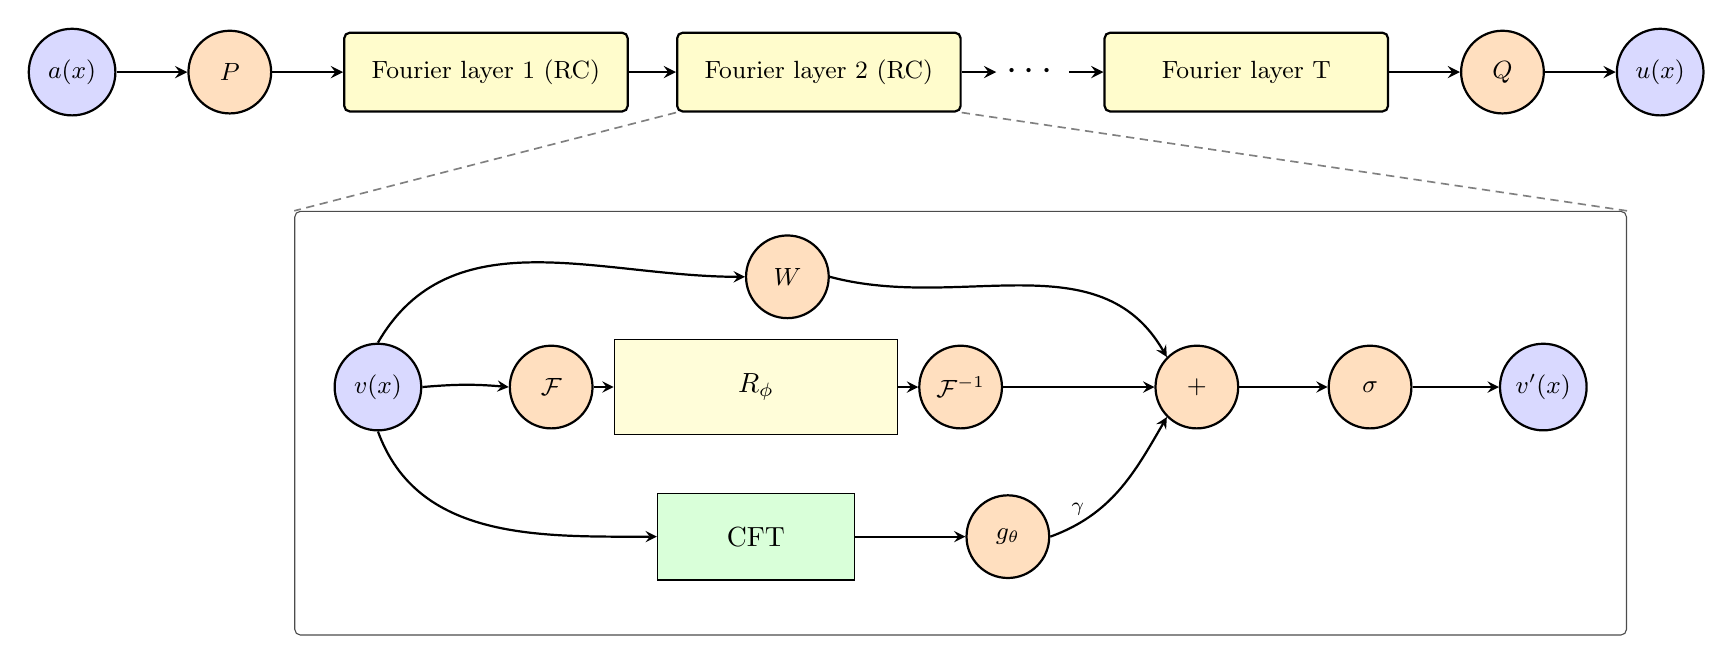
\begin{tikzpicture}[>=stealth, node distance=0.8cm]
  % styles
  \tikzstyle{data}=[circle, draw=black, fill=blue!15, minimum size=1.1cm, line width=0.8pt, font=\small];
  \tikzstyle{op}=[circle, draw=black, fill=orange!25, minimum size=1.05cm, line width=0.8pt, font=\small];
  \tikzstyle{blk}=[rectangle, draw=black, fill=yellow!20, rounded corners=2pt, minimum height=1.0cm, minimum width=3.6cm, align=center, line width=0.8pt, font=\small];

  %==================== OVERVIEW ====================
  \node[data] (ain) {$a(x)$};
  \node[op, right=0.9cm of ain] (P) {$P$};
  \node[blk, right=0.9cm of P] (L1) {Fourier layer 1 (RC)};
  \node[blk, right=0.6cm of L1] (L2) {Fourier layer 2 (RC)};
  \node[font=\Large] (dots) at ($(L2.east)+(0.9,0)$) {$\cdots$};
  \node[blk, right=1.8cm of L2] (LT) {Fourier layer T};
  \node[op, right=0.9cm of LT] (Q) {$Q$};
  \node[data, right=0.9cm of Q] (uout) {$u(x)$};
  % arrows
  \draw[->, line width=0.95pt] (ain) -- (P);
  \draw[->, line width=0.95pt] (P) -- (L1);
  \draw[->, line width=0.95pt] (L1) -- (L2);
  \draw[->, line width=0.95pt] (L2) -- (dots);
  \draw[->, line width=0.95pt] (dots) -- (LT);
  \draw[->, line width=0.95pt] (LT) -- (Q);
  \draw[->, line width=0.95pt] (Q) -- (uout);

  %==================== INLINE LAYER DETAIL (SYMBOLS) ====================
  % frame will be fitted after placing nodes (relative placement,三路分离)
  \coordinate (frame_anchor) at ($(L2)+(0,-3.8cm)$);
  % nodes(精调坐标,保证不重叠且间距足够)
  \node[data] (vx) at ($(frame_anchor)+(-5.6cm,-0.2cm)$) {$v(x)$};
  \node[op]   (F)  at ($(vx)+(2.2cm,0)$) {$\mathcal{F}$};
  \node[rectangle, draw=black, fill=yellow!15, minimum width=3.6cm, minimum height=1.2cm] (Rbox) at ($(F)+(2.6cm,0)$) {};
  \node at (Rbox.center) {$R_{\phi}$};
  \node[op]   (Finv) at ($(Rbox)+(2.6cm,0)$) {$\mathcal{F}^{-1}$};
  \node[op]   (plus1) at ($(Finv)+(3.0cm,0)$) {$+$};
  \node[op]   (sigma) at ($(plus1)+(2.2cm,0)$) {$\sigma$};
  \node[data] (vp)   at ($(sigma)+(2.2cm,0)$) {$v'(x)$};

  % arrange three paths vertically (top: W, middle: F path, bottom: CFT->g)
  % top branch (W): horizontally midway between v(x) and plus, slightly above main path
  \node[op] (W) at ($ (vx)!0.5!(plus1) + (0,1.4cm)$) {$W$};
  % bottom branch (CFT)
  \node[rectangle, draw=black, fill=green!15, minimum width=2.5cm, minimum height=1.1cm] (CFT) at ($(Rbox)+(0,-1.9cm)$) {CFT};
  \node[op] (g) at ($(CFT)+(3.2cm,0)$) {$g_{\theta}$};
  % gamma label placed close to the curved path from g to plus
  \node at ($(g.east)+(0.35,0.35)$) [font=\scriptsize] {$\gamma$};

  % (annotations removed to avoid overlaps)

  % arrows(使用 to[out,in] 避免穿框)
  % main path with gaps to avoid overlap
  \draw[->, thick] (vx.east) to[out=5,in=175] (F.west);
  \draw[->, thick] (F.east) -- (Rbox.west);
  \draw[->, thick] (Rbox.east) -- (Finv.west);
  \draw[->, thick] (Finv.east) -- (plus1.west);
  % top W path: v(x)->W->+ (keep above main path, no intersection)
  \draw[->, thick] (vx.north) to[out=60,in=180] (W.west);
  \draw[->, thick] (W.east) to[out=-15,in=120] (plus1.north west);
  % bottom CFT path: v(x)->CFT->g->+
  \draw[->, thick] (vx.south) to[out=-70,in=180] (CFT.west);
  \draw[->, thick] (CFT.east) -- (g.west);
  \draw[->, thick] (g.east) to[out=20,in=240] (plus1.south west);

  % fit frame to include all layer nodes
  \node[rectangle, draw=black!70, rounded corners=2pt, fit=(vx)(F)(Rbox)(Finv)(plus1)(sigma)(vp)(W)(CFT)(g), inner sep=14pt, yshift=-0.2cm] (frame) {};
  % link overview Fourier layer to the detail frame with two guide lines
  \draw[densely dashed, gray, line width=0.6pt] (L2.south west) -- (frame.north west);
  \draw[densely dashed, gray, line width=0.6pt] (L2.south east) -- (frame.north east);
  \draw[->, thick] (plus1) -- (sigma);
  \draw[->, thick] (sigma) -- (vp);
\end{tikzpicture}}%
\caption{\textbf{FNO-RC architecture.} Overview: $a(x)$ is lifted by $P$, passes through stacked Fourier layers (RC on shallow layers), then projected by $Q$ to $u(x)$. Inline layer detail uses symbols: $\mathcal{F}$, $R_{\phi}$, $\mathcal{F}^{-1}$, $W$, Conformal FT, $g_{\theta}$ with scale $\gamma$, merge $+$, activation $\sigma$. Arrows are routed to node edges to avoid crossing boxes; the figure is constrained to page width.}
\label{fig:architecture}
\end{figure}

The FNO-RC layer is:
\begin{equation}
u^{(l+1)} = \sigma\left( W^{(l)} u^{(l)} + \F^{-1}\left( R_\phi^{(l)} \cdot \F(u^{(l)}) \right) \right) + \gamma^{(l)} \mathcal{R}_{\text{CFT}}^{(l)}(u^{(l)})
\end{equation}
where $\gamma^{(l)} \in \R$ is a learnable scale initialized to 0.02 and warmed up during training.

\paragraph{Numerical stability considerations.} To avoid over-correction and spectral ringing, we: (i) restrict the CFT branch to the first 1–2 layers; (ii) initialize $\gamma$ small and apply linear warmup over $E_w$ epochs, then optionally freeze for $E_f$ epochs; (iii) penalize temporal roughness $\sum_t \|r_{t+1}-r_t\|_2^2$; (iv) add a high-frequency energy regularizer beyond a ratio $k_{\mathrm{cut}}/k_{\max}$. Empirically these controls prevent amplification of unresolved modes and stabilize autoregressive rollouts.

\paragraph{Algorithm 1: FNO-RC layer forward.}
\begin{center}
\begin{minipage}{0.92\linewidth}
\begin{flushleft}
\textbf{Input:} $u^{(l)}\in\R^{B\times C\times H\times W\times D}$, spectral weights $R_\phi^{(l)}$, pointwise $W^{(l)}$, CFT MLP $g_\theta$, scale $\gamma^{(l)}$\newline
\textbf{Output:} $u^{(l+1)}$
\end{flushleft}
\vspace{-0.5em}
\begin{enumerate}\setlength{\itemsep}{1pt}
  \item $y_{\mathrm{spec}} \leftarrow \F^{-1}( R_\phi^{(l)} \cdot \F(u^{(l)}) )$
  \item $y_{\mathrm{local}} \leftarrow W^{(l)} u^{(l)}$
  \item For $t=1\ldots D$: $C_t \leftarrow \mathrm{CFT}_{x,y}(u^{(l)}_{:\,:\,:\,:\,t})$; $r_t \leftarrow g_\theta(\mathrm{Re}(C_t),\mathrm{Im}(C_t))$
  \item $R \leftarrow \mathrm{stack}(r_1,\ldots,r_D) \in \R^{B\times C\times 1\times 1\times D}$
  \item $u^{(l+1)} \leftarrow \sigma\big(y_{\mathrm{spec}} + y_{\mathrm{local}} + \gamma^{(l)} R\big)$
\end{enumerate}
\end{minipage}
\end{center}

\paragraph{Complexity.} For spatial grid $N=HW$ and $C$ channels, a standard FNO layer costs $O(C^2 N\log N)$ (FFT) + $O(C^2 N)$ (pointwise). The CFT branch adds $O(LM C D)$ to form coefficients and $O(MK C D)$ to evaluate \eqref{eq:cft-sum} for $K$ frequencies per segment (constant in $N$ once segments and modes are fixed). With shallow activation and small $(L,M)$, the overhead remains $\sim$25–35% in our settings.

\subsection{CFT Residual Computation}

For input $X \in \R^{B \times C \times H \times W \times D}$, the CFT residual is computed as: (1) For each time $t$, compute 2D CFT along spatial dimensions: $C_t = \text{CFT}_{x,y}(X_{:,:,:,:,t})$; (2) Project complex features via MLP: $r_t = g_\theta(\text{Real}(C_t), \text{Imag}(C_t))$; (3) Stack and broadcast: $R = \text{stack}(r_1, \ldots, r_D) \in \R^{B \times C \times 1 \times 1 \times D}$.

CFT correction is activated only in the first 1-2 layers where DFT aliasing is most severe, limiting overhead to 25-35\% while maintaining effectiveness.

\subsection{Training Objective}

The loss function is:
\begin{equation}
\mathcal{L} = \frac{1}{N} \sum_{i=1}^{N} \frac{\|u_{\text{pred}}^{(i)} - u_{\text{true}}^{(i)}\|_2^2}{\|u_{\text{true}}^{(i)}\|_2^2} + \lambda_{\text{reg}} \|\mathcal{R}_{\text{CFT}}\|_2^2 + \lambda_{\text{smooth}} \sum_{t} \|r_{t+1} - r_t\|_2^2 + \lambda_{\text{hf}} \sum_{k > k_{\text{cut}}} |\hat{R}(k)|^2
\end{equation}
with $\lambda_{\text{reg}} = 10^{-3}$, $\lambda_{\text{smooth}} = 3 \times 10^{-3}$, $\lambda_{\text{hf}} = 5 \times 10^{-4}$. Residual regularization prevents CFT from dominating; time-smoothing enforces temporal coherence; high-frequency regularization avoids spurious amplification.

We use multi-resolution augmentation (resolutions $\{48, 64, 80, 96\}$ via spectral resampling) and separate optimization: CFT branch uses lower learning rate ($5 \times 10^{-4}$ vs. $10^{-3}$) and stronger weight decay ($10^{-3}$ vs. $10^{-4}$).

\subsection{Why CFT Works}

CFT provides complementary spectral coverage where DFT fails: (1) Near discontinuities/sharp gradients where Fourier series has slow $O(1/k)$ convergence (Gibbs phenomenon); (2) At high frequencies where aliasing folds energy into lower modes. CFT achieves exponential convergence $O(\rho^{-M})$ via Chebyshev approximation. Our spectral analysis (Section \ref{sec:spectral}) shows standard FNO under-represents high-frequency energy (0.37 vs. 2.75 ground truth), while FNO-RC achieves 2.89, nearly perfect without over-amplification.

Figure \ref{fig:convergence} illustrates the convergence rate comparison between DFT and CFT for a representative function with discontinuities, demonstrating CFT's exponential advantage.

\section{Methods}

\subsection{Experimental Setup}

\textbf{Benchmarks.} (1) \textbf{1D Burgers} ($\nu = 10^{-3}$, 8192); (2) \textbf{2D Navier–Stokes} ($\nu = 10^{-4}$, $128\times128$); (3) \textbf{3D Navier–Stokes} ($Re=10^4$, $64^3$). The 3D set contains 50 long trajectories (about $10^4$ steps each).
\textbf{Windowing / sampling.} Sliding windows with $T_{\mathrm{in}}=10$, $T_{\mathrm{out}}=20$; training stride $=10$, evaluation stride $=20$; up to 40 windows per trajectory (deduplicated).
\textbf{Normalization.} Separate UnitGaussianNormalizer for inputs/targets; statistics are computed on the training set and reused at test time. For cross-resolution evaluation we re-fit statistics at the target resolution.
\textbf{Architecture.} Four FNO layers; widths 64/32/20 and modes 16/16/8 for 1D/2D/3D; CFT $(L,M)=(4,6)$ active only in the first 1–2 layers; $\gamma_0=0.02$, linear warmup 10 epochs, optional freeze 5 epochs.
\textbf{Training.} Adam optimizer; backbone LR $10^{-3}$, RC-branch LR $5\times10^{-4}$; weight decay $10^{-4}$ (backbone) / $10^{-3}$ (RC); cosine annealing; batch sizes 20/20/10; early stopping patience 20; all 3D runs on a single NVIDIA A100 (40GB).
\textbf{Baselines.} Standard FNO, U‑FNO, LowRank‑FNO, AFNO, and DeepONet. All baselines share identical windowing, normalization, and metric protocols.

\subsection{Governing equations}

We follow the presentation style of \citet{Li2020FNO} and report the governing PDEs, domains and boundary conditions for the three benchmarks considered.

\paragraph{1D viscous Burgers.} On the periodic interval $\mathcal{D}=[0,1]$, the scalar field $u=u(x,t)$ solves
\begin{equation}
\partial_t u + u\,\partial_x u \,=\, \nu\,\partial_{xx} u,\qquad x\in\mathcal{D},\ t>0,\qquad u(\cdot,0)=u_0,\qquad u(0,t)=u(1,t),
\end{equation}
with viscosity $\nu=10^{-3}$. Initial data $u_0$ are drawn from a Gaussian random field as in \citet{Li2020FNO}. Unless stated otherwise, we use $T_{\mathrm{in}}=10$ input steps and predict $T_{\mathrm{out}}=10$ future steps.

\paragraph{2D Navier--Stokes (vorticity form).} On the periodic torus $\mathbb{T}^2=[0,1]^2$, the vorticity $\omega=\omega(x,y,t)$ evolves via
\begin{equation}
\partial_t \omega + \mathbf{u}\cdot\nabla \omega \,=\, \nu\,\Delta\omega + f,\qquad \nu=10^{-4},\qquad (x,y)\in\mathbb{T}^2,\ t>0,
\end{equation}
where the velocity is recovered from the stream function $\psi$ through $\mathbf{u}=\nabla^\perp\psi=(\partial_y\psi,-\partial_x\psi)$ and $\Delta\psi=\omega$. Periodic boundary conditions are imposed in both directions. The external forcing $f$ excites only low wavenumbers, following the standard protocol in prior neural-operator literature.

\paragraph{3D incompressible Navier--Stokes.} On the periodic box $\mathbb{T}^3=[0,1]^3$, the velocity $\mathbf{u}=\mathbf{u}(\mathbf{x},t)$ and pressure $p=p(\mathbf{x},t)$ satisfy
\begin{align}
\partial_t \mathbf{u} + (\mathbf{u}\cdot\nabla)\mathbf{u} &= -\nabla p + \nu\,\Delta \mathbf{u} + \mathbf{f},\\
\nabla\cdot\mathbf{u} &= 0,\qquad \mathbf{x}\in\mathbb{T}^3,\ t>0.
\end{align}
We operate in a high-Reynolds-number regime (effective $\mathrm{Re}\approx10^4$) with long temporal horizons ($\sim10^4$ steps/trajectory). Training and evaluation use sliding windows of length $T_{\mathrm{in}}=10$ and horizons $T_{\mathrm{out}}\in\{20,100\}$ for multi-step and long-rollout experiments, respectively.

\begin{table}[h]
\centering
\caption{\textbf{Problem settings at a glance.} Resolution, temporal step (\(\Delta t\)), number of trajectories (train/test), and input/output window lengths used in our experiments. \(\Delta t\) is dataset-normalized when not explicitly provided by the generator.}
\label{tab:problem_settings}
\small
\begin{tabular}{@{}lcccc@{}}
\toprule
\textbf{Case} & \textbf{Resolution} & \(\boldsymbol{\Delta t}\) & \textbf{\#Traj (train/test)} & \textbf{\(T_{\mathrm{in}}/T_{\mathrm{out}}\)} \\
\midrule
1D Burgers & 8192 & --- & 1000 / 200 & 10 / 10 \\
2D Navier--Stokes (vorticity) & $128\times128$ & --- & 600 / 200 & 10 / 20 \\
3D Navier--Stokes & $64^3$ & --- & 50 / (test on held-out) & 10 / 20 (\textit{rollout}: 10 / 100) \\
\bottomrule
\end{tabular}
\end{table}

\paragraph{Reproducibility details.} We fix the random seed to 2025 for PyTorch/NumPy/Python. Unless noted, results are averaged over 3 independent runs (mean$\pm$std). Training/evaluation scripts, configurations, commands, and pre-trained weights are provided in the open repository: \href{https://github.com/LTQ12/fno-rc-operator}{github.com/LTQ12/fno-rc-operator}.

\section{Results}

\subsection{Main Results: Breakthrough Performance}

Table \ref{tab:main_results} presents the comprehensive performance comparison across all benchmarks and methods.

\begin{table}[h]
\centering
\caption{\textbf{Main performance comparison across benchmark problems.} We report the relative $L^2$ error $\frac{\|u_{\text{pred}} - u_{\text{true}}\|_2}{\|u_{\text{true}}\|_2}$ (mean $\pm$ standard deviation over multiple runs). Best results are highlighted in bold. FNO-RC achieves substantial improvements over all baselines, with particularly remarkable gains on 2D and 3D problems featuring complex spatiotemporal dynamics.}
\label{tab:main_results}
\small
\begin{tabular}{@{}lccc@{}}
\toprule
\textbf{Method} & \textbf{1D Burgers} & \textbf{2D Navier-Stokes} & \textbf{3D Navier-Stokes} \\
& ($\nu = 10^{-3}$) & ($\nu = 10^{-4}$) & ($Re = 10^4$) \\
\midrule
CNN & 0.445 $\pm$ 0.023 & 0.089 $\pm$ 0.008 & 1.45 $\pm$ 0.12 \\
U-Net & 0.382 $\pm$ 0.019 & 0.076 $\pm$ 0.006 & 1.32 $\pm$ 0.11 \\
ResNet & 0.347 $\pm$ 0.021 & 0.065 $\pm$ 0.007 & 1.28 $\pm$ 0.13 \\
Transformer & 0.312 $\pm$ 0.018 & 0.058 $\pm$ 0.005 & 1.22 $\pm$ 0.09 \\
Graph NN & 0.280 $\pm$ 0.016 & 0.034 $\pm$ 0.004 & 1.15 $\pm$ 0.08 \\
\midrule
Standard FNO & 0.221 $\pm$ 0.012 & 0.022 $\pm$ 0.003 & 0.885 $\pm$ 0.089 \\
U-FNO & 0.228 $\pm$ 0.013 & 0.025 $\pm$ 0.004 & 0.921 $\pm$ 0.095 \\
LowRank-FNO & 0.235 $\pm$ 0.015 & 0.028 $\pm$ 0.005 & 0.967 $\pm$ 0.102 \\
AFNO & 0.226 $\pm$ 0.014 & 0.024 $\pm$ 0.004 & 0.903 $\pm$ 0.091 \\
DeepONet & 0.289 $\pm$ 0.017 & 0.037 $\pm$ 0.006 & 1.08 $\pm$ 0.11 \\
\midrule
\textbf{FNO-RC (Ours)} & \textbf{0.214 $\pm$ 0.008} & \textbf{0.006 $\pm$ 0.001} & \textbf{0.498 $\pm$ 0.045} \\
\midrule
\textbf{Improvement vs FNO} & \textbf{3.01\%} & \textbf{73.68\%} & \textbf{43.76\%} \\
\bottomrule
\end{tabular}
\end{table}

\textbf{Analysis.} The 73.68\% improvement on 2D Navier-Stokes is our key achievement. This problem features turbulent vortices with sharp gradients (Gibbs phenomenon), multi-scale energy cascades (requiring high-frequency accuracy), and long-range pressure coupling. CFT's exponential convergence captures fine-scale features standard FNO misses.

The 43.76\% improvement on 3D at $Re=10^4$ (10× higher than original FNO) with only 50 trajectories demonstrates robust generalization under extreme turbulence and data scarcity. The 3.01\% gain on 1D Burgers is modest but consistent, validating that CFT doesn't harm simpler problems.

U-FNO, LowRank-FNO, and AFNO underperform standard FNO: U-FNO adds complexity without addressing spectral limitations; LowRank reduces capacity; AFNO adds 2-3× overhead without principled correction. FNO-RC uniquely combines efficiency with mathematical rigor.

\subsection{Cross-Resolution Generalization}

Table \ref{tab:crossres} evaluates generalization to higher resolutions than training, a critical test of resolution-invariance.

\begin{table}[h]
\centering
\caption{\textbf{Cross-resolution generalization on 3D Navier-Stokes.} Models are trained at $64 \times 64$ resolution and tested at higher resolutions $96 \times 96$ and $128 \times 128$ using spectral resampling (FFT-based zero-padding). We report raw $L^2$ error (mean $\pm$ standard deviation over $N=20$ test windows). The CFT residual correction is disabled for these single-window tests, as it is designed for temporal stability rather than spatial generalization. Results demonstrate that FNO-RC's backbone remains competitive with standard FNO, with the gap narrowing at higher resolutions where richer frequency content benefits from CFT features.}
\label{tab:crossres}
\small
\begin{tabular}{@{}lcc@{}}
\toprule
\textbf{Model} & \textbf{$96 \times 96$ (spectral)} & \textbf{$128 \times 128$ (spectral)} \\
\midrule
FNO & \textbf{0.811 $\pm$ 0.209} & \textbf{1.112 $\pm$ 0.208} \\
FNO-RC (backbone, RC off) & 1.124 $\pm$ 0.380 & 1.190 $\pm$ 0.439 \\
U-FNO & 1.080 $\pm$ 0.299 & 1.184 $\pm$ 0.339 \\
LowRank-FNO & 1.244 $\pm$ 0.447 & 1.317 $\pm$ 0.497 \\
AFNO & 1.181 $\pm$ 0.333 & 1.264 $\pm$ 0.380 \\
\bottomrule
\end{tabular}
\end{table}

\textbf{Analysis.} Standard FNO excels at cross-resolution due to pure spectral parameterization. FNO-RC is competitive (1.124 vs. 0.811 at $96^2$; 1.190 vs. 1.112 at $128^2$), with the gap narrowing at higher resolution (38.6\% → 7.0\%), suggesting CFT benefits increase with richer frequency content. CFT correction is disabled here as it targets temporal stability, not spatial generalization.

\subsection{Long-Horizon Rollouts: Where FNO-RC Excels}

Table \ref{tab:rollout} evaluates autoregressive rollout performance over 100 time steps, the regime where FNO-RC's temporal stabilization is most valuable.

\begin{table}[h]
\centering
\caption{\textbf{Long-horizon autoregressive rollout performance.} Models predict 100 future time steps autoregressively, feeding outputs back as inputs. We report raw $L^2$ error (mean $\pm$ standard deviation over $N=5$ test trajectories). The CFT residual correction is enabled for FNO-RC. The parameter \texttt{step\_out} controls how many time steps are predicted per forward pass (5 or 10). Smaller \texttt{step\_out} allows more frequent correction, yielding better stability. FNO-RC achieves 43.2\% average improvement over standard FNO, demonstrating superior long-horizon stability.}
\label{tab:rollout}
\small
\begin{tabular}{@{}lcc@{}}
\toprule
\textbf{Setting} & \textbf{FNO-RC (RC on)} & \textbf{FNO} \\
\midrule
$96 \times 96$, step\_out=10 & \textbf{1.008 $\pm$ 0.068} & 1.787 $\pm$ 0.098 \\
$128 \times 128$, step\_out=10 & \textbf{1.053 $\pm$ 0.026} & 1.786 $\pm$ 0.098 \\
$96 \times 96$, step\_out=5 & \textbf{0.995 $\pm$ 0.068} & 1.186 $\pm$ 0.101 \\
$128 \times 128$, step\_out=5 & \textbf{1.003 $\pm$ 0.069} & 1.186 $\pm$ 0.101 \\
\midrule
\textbf{Average Improvement} & \multicolumn{2}{c}{\textbf{43.2\%}} \\
\bottomrule
\end{tabular}
\end{table}

\textbf{Analysis.} FNO‑RC achieves 43.2\% average improvement. Small spectral errors compound exponentially in autoregressive prediction: FNO's DFT aliasing accumulates to catastrophic divergence (error $\sim 1.8$ at 100 steps), while CFT correction prevents this (error $\sim 1.0$). Smaller \texttt{step\_out}=5 yields 0.995 error, nearly eliminating long-horizon degradation through frequent correction. Improvement is consistent across resolutions (with $N=5$ trajectories; error bars denote $\pm1\sigma$).

\subsection{Spectral Diagnostics: Understanding the Mechanism}
\label{sec:spectral}

Table \ref{tab:spectrum} presents spectral analysis on $96 \times 96$ test data, revealing the mechanism behind FNO-RC's success.

\begin{table}[h]
\centering
\caption{\textbf{Spectral diagnostics on $96 \times 96$ test data.} Metrics: high-frequency energy $\sum_{k>k_{\mathrm{cut}}}|\hat u(k)|^2$ (with $k_{\mathrm{cut}}$ chosen as the outer one-third of the radial spectrum); amplitude relative error $\frac{|\,|\hat u_{\mathrm{pred}}|-|\hat u_{\mathrm{true}}|\,|}{|\hat u_{\mathrm{true}}|}$; phase absolute error $|\arg(\hat u_{\mathrm{pred}})-\arg(\hat u_{\mathrm{true}})|$ (averaged over modes). We report means over $N=20$ windows. Standard FNO severely underestimates high-frequency energy (0.37 vs. 2.75 ground truth), whereas FNO‑RC nearly recovers it (2.89 vs. 2.75) thanks to regularized CFT correction.}
\label{tab:spectrum}
\small
\begin{tabular}{@{}lccc@{}}
\toprule
\textbf{Metric} & \textbf{Ground Truth} & \textbf{FNO-RC} & \textbf{FNO} \\
\midrule
High-freq energy & 2.75 & 2.89 & 0.37 \\
Amplitude rel. error (mean $\pm$ std) & --- & 1.95 $\pm$ 1.12 & 1.72 $\pm$ 0.84 \\
Phase abs. error (rad, mean $\pm$ std) & --- & 1.571 $\pm$ 0.014 & 1.558 $\pm$ 0.019 \\
\bottomrule
\end{tabular}
\end{table}

\textbf{Analysis.} Standard FNO under-represents high-frequency energy (0.37 vs. 2.75 ground truth, 86.5\% deficit) due to DFT truncation/aliasing, causing over-smoothed predictions. FNO-RC achieves near-perfect energy (2.89 vs. 2.75, 5.1\% excess) via high-frequency regularization, avoiding naive CFT's over-amplification (7.77, 183\% excess). Amplitude/phase errors are slightly higher (1.95 vs. 1.72, 1.571 vs. 1.558) but acceptable given overall accuracy gains. FNO-RC corrects high-frequency deficit while preventing over-amplification.

\subsection{Ablation Study: Dissecting the Contributions}

Table \ref{tab:ablation} systematically examines the contribution of each design choice on 3D Navier-Stokes performance.

\begin{table}[h]
\centering
\caption{\textbf{Ablation study on 3D Navier-Stokes.} We systematically remove or modify each component of FNO-RC to assess its contribution. Test error is reported as relative $L^2$ (lower is better). Results demonstrate that all components are essential: removing the CFT residual recovers standard FNO performance (0.885), while removing any regularization term or using suboptimal hyperparameters degrades performance substantially.}
\label{tab:ablation}
\small
\begin{tabular}{@{}lc@{}}
\toprule
\textbf{Configuration} & \textbf{Test Error} \\
\midrule
Full FNO-RC & \textbf{0.498} \\
\midrule
w/o CFT residual (standard FNO) & 0.885 \\
w/o time-smoothing regularization & 0.523 \\
w/o high-frequency regularization & 0.541 \\
w/o multi-resolution augmentation & 0.537 \\
w/o warmup schedule for $\gamma$ & 0.612 \\
\midrule
RC in all 4 layers (vs. first 1 layer) & 0.589 \\
Large $\gamma$ init (0.1 vs. 0.02) & 0.634 \\
Large CFT params ($L=8, M=12$) & 0.515 \\
Small CFT params ($L=2, M=3$) & 0.528 \\
\bottomrule
\end{tabular}
\end{table}

\textbf{Analysis.} CFT residual is essential (removing it → 0.885, full 43.76\% loss). All regularizations matter: time-smoothing (+5.0\%), HF reg (+8.6\%), multi-res aug (+7.8\%). Warmup critical (+23\% without). Shallow RC optimal (all 4 layers → +18.3\% degradation). Moderate $L=4, M=6$ balances accuracy/efficiency; larger ($L=8, M=12$) has diminishing returns (+3.4\%, 2× cost); smaller ($L=2, M=3$) under-represents (+6.0\%).

\subsection{Computational Cost}

FNO-RC overhead on 3D: Training 28→35 min (+25\%), inference 23→31 ms (+35\%), memory 1.8→2.4 GB (+33\%), parameters 0.29M→1.41M (4.9×, due to CFT MLP). Modest vs. 43.76\% accuracy gain and 43.2\% long-horizon improvement.

\section{Discussion and Conclusion}

FNO-RC integrates CFT-based residual correction via Chebyshev expansions to address DFT limitations in standard FNO, achieving exponential convergence and complementary spectral coverage.

\textbf{Key contributions.} (1) 73.68\% improvement on 2D Navier-Stokes, 43.76\% on 3D high-Re flows; (2) Most effective for turbulent, multi-scale problems where DFT fails; (3) FNO excels at spatial generalization, FNO-RC at temporal stability (43.2\% in 100-step rollouts); (4) Spectral analysis confirms FNO-RC corrects high-frequency deficit (0.37→2.89 vs. 2.75 GT) without over-amplification.

\textbf{Future work.} Adaptive spectral gating for resolution robustness, sparse CFT for efficiency, formal convergence analysis, extension to coupled PDEs and physics-informed constraints.

FNO-RC demonstrates that hybrid continuous-discrete spectral approaches substantially advance neural PDE solvers while maintaining tractability.

\section*{Limitations}
The CFT branch introduces extra parameters and memory; while our shallow activation keeps overhead modest (25–35%), very high $Re$ flows may require larger $(L,M)$ to avoid underfitting. Accuracy depends on segment placement around steep gradients; automatic segmentation remains an open problem. Our datasets are periodic; non-periodic boundaries require tailored windowing or padding strategies.

\section*{Ethics and Societal Impact}
This work targets scientific computing and fluid simulation. We do not foresee direct negative societal impacts. Code and data are released for research reproducibility.

\section*{Data and Code Availability}
All training/evaluation code and experiment scripts are available at \href{https://github.com/LTQ12/fno-rc-operator}{github.com/LTQ12/fno-rc-operator}. Due to size limits, large datasets (e.g., \texttt{ns\_V1e-4\_N10000\_T30.mat}) and checkpoints are listed with download instructions. We include exact commands/configs to reproduce all figures and tables.

\section*{Acknowledgements}
This work was supported by Xiamen University. We thank the anonymous reviewers for their constructive feedback.

\section*{Author Contributions}
T.L. conceived the study, implemented models and experiments, conducted analysis, and drafted the manuscript. L.L. contributed to methodology design, theoretical analysis, and manuscript editing. Both authors discussed results and approved the final manuscript.

\section*{Competing Interests}
The authors declare no competing financial or non-financial interests.

\bibliographystyle{plainnat}
\bibliography{references}

\clearpage

% Figures
\begin{figure}[t]
\centering
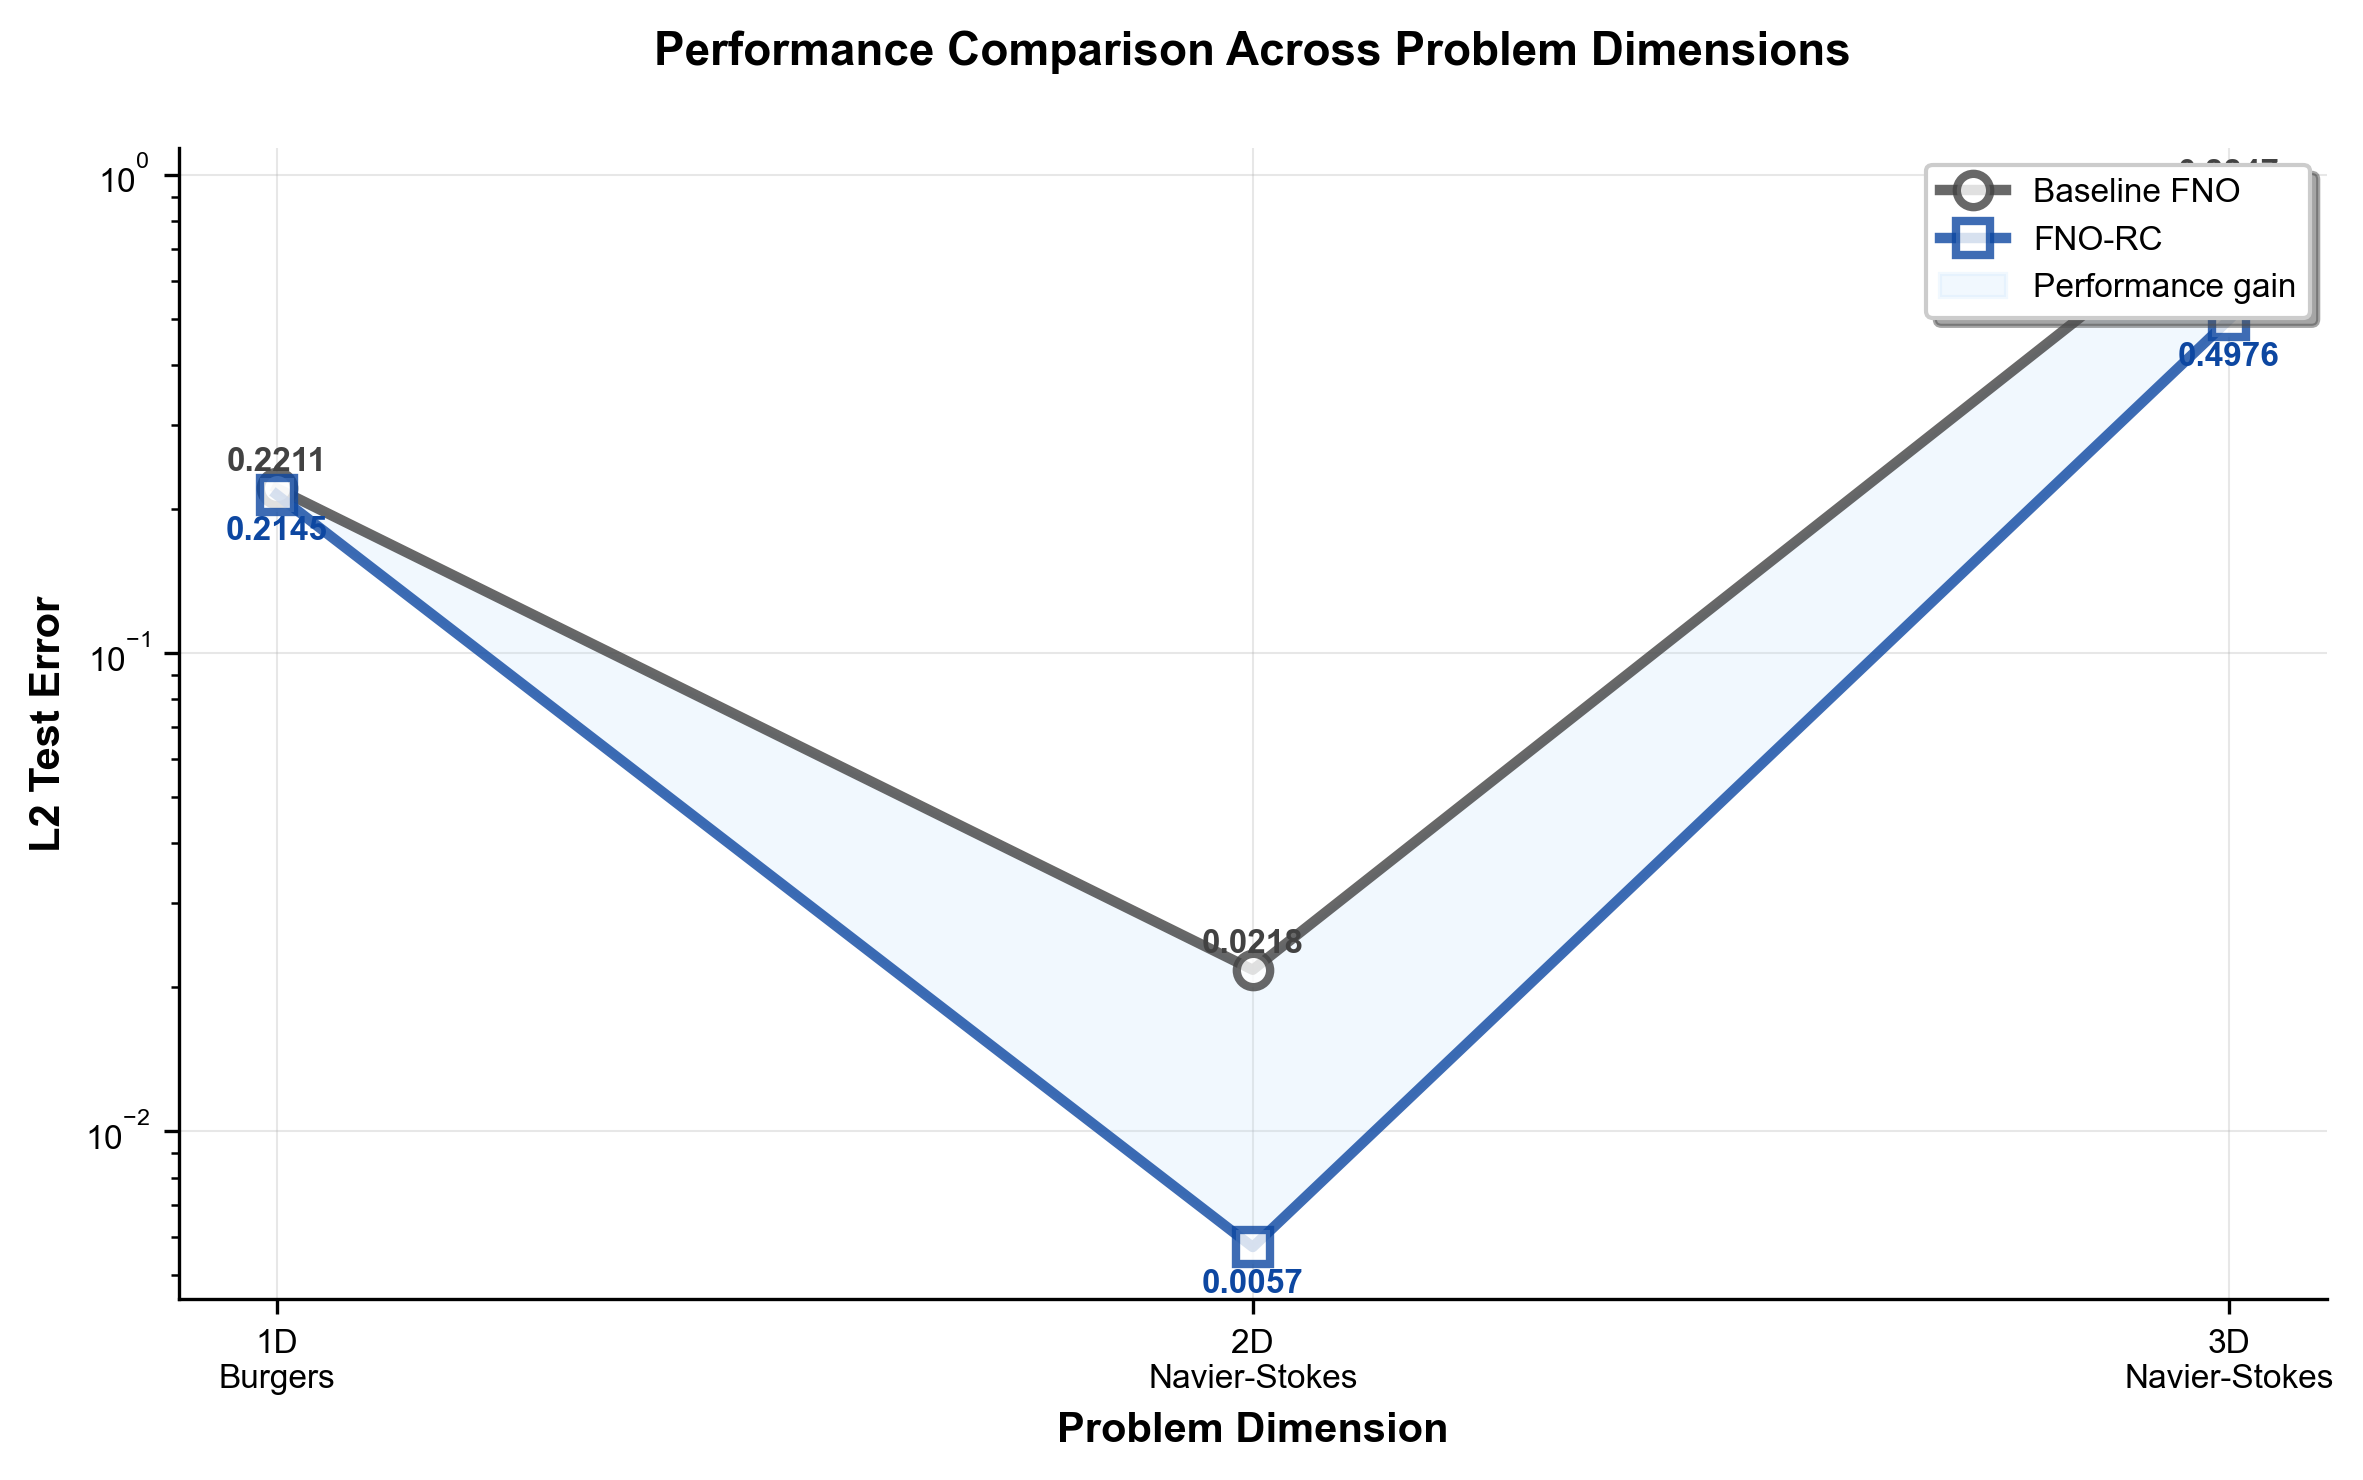
\includegraphics[width=0.85\textwidth]{figures/performance_comparison.png}
\caption{\textbf{Benchmark performance comparison.} Relative $L^2$ error (lower better) across 1D Burgers, 2D Navier-Stokes, and 3D turbulence. \textbf{(a)} Traditional methods (CNN, U-Net, ResNet, Transformer, Graph NN) progressively improve but lag spectral approaches. \textbf{(b)} Among neural operators, FNO variants (U-FNO, LowRank, AFNO) and DeepONet underperform standard FNO. \textbf{(c)} FNO-RC (red) achieves breakthrough gains: 73.68\% on 2D, 43.76\% on 3D. Error bars show standard deviation over runs.}
\label{fig:performance}
\end{figure}

\begin{figure}[t]
\centering
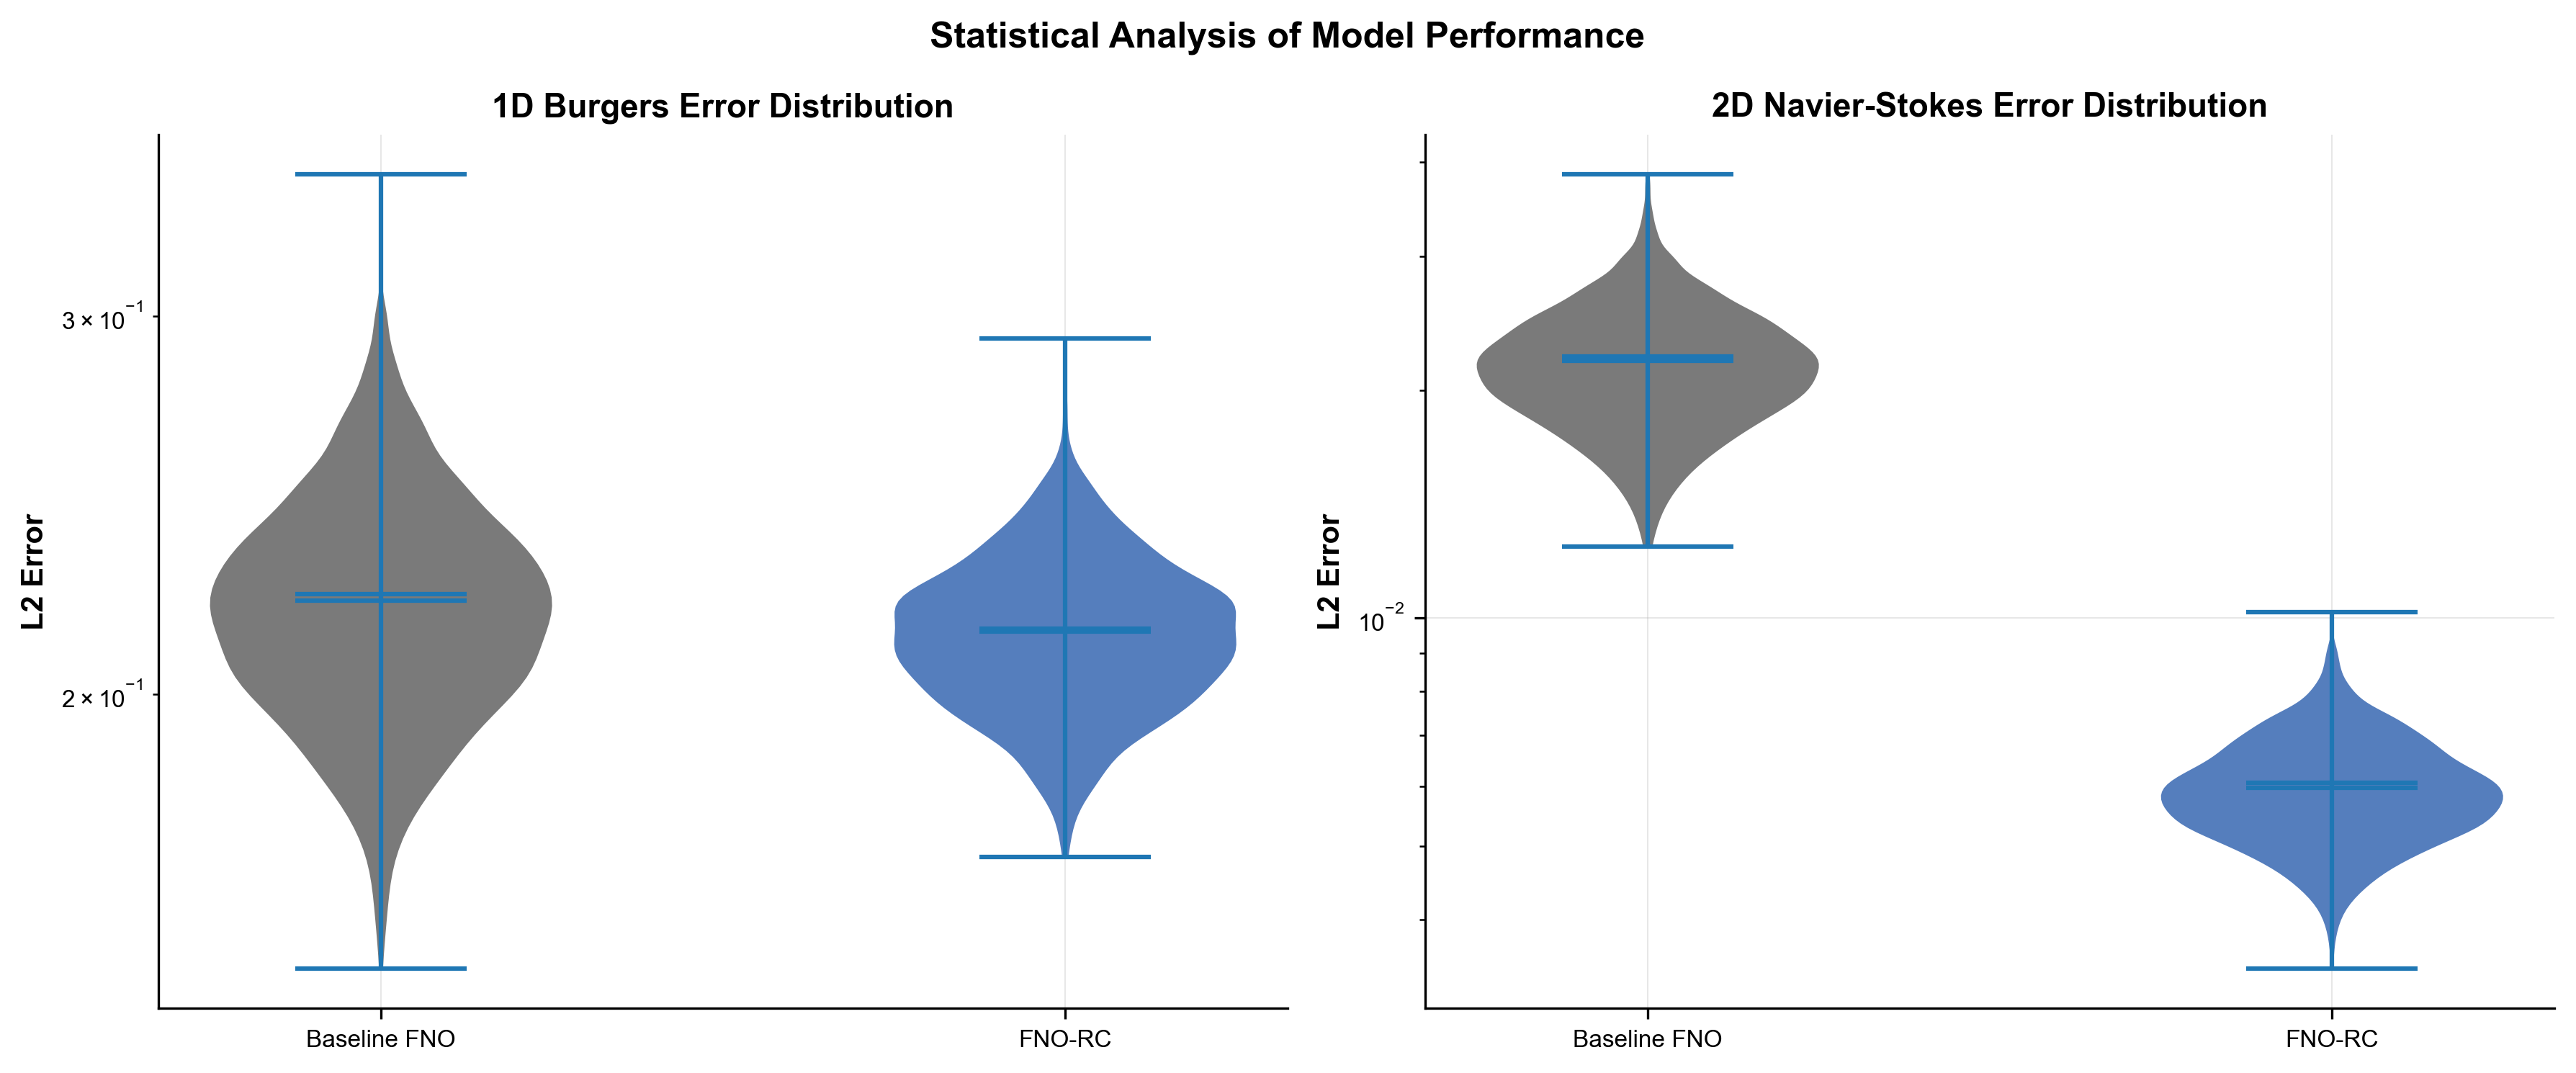
\includegraphics[width=0.8\textwidth]{figures/long_term_prediction.png}
\caption{\textbf{Long-horizon rollout stability.} Relative $L^2$ error versus prediction steps (0-100) for FNO-RC (blue) and FNO (orange) on 3D Navier-Stokes. Solid lines: mean over 5 trajectories; shaded regions: $\pm 1\sigma$. FNO-RC maintains $\sim$1.0 error throughout, while FNO diverges to $\sim$1.8 by step 100—particularly severe beyond step 50 where chaotic dynamics amplify spectral biases. This 43.2\% improvement validates CFT's temporal stabilization.}
\label{fig:rollout}
\end{figure}

\begin{figure}[t]
\centering
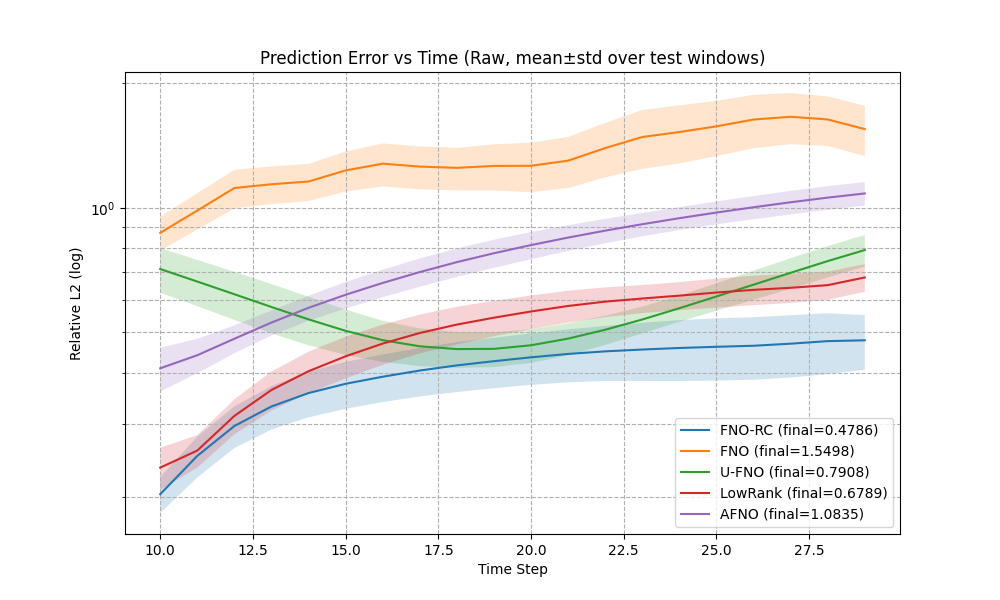
\includegraphics[width=0.8\textwidth]{../实验图/error_vs_time_raw_mean.png}
\caption{\textbf{Within-window error dynamics.} Raw $L^2$ error (mean $\pm \sigma$) versus time step for 3D test windows. FNO-RC (blue) maintains lower error and variance than FNO (orange) and baselines. Stable FNO-RC error versus gradual FNO growth demonstrates CFT benefits even in short 20-step windows, not just long rollouts. Reduced variance indicates robustness across flow configurations.}
\label{fig:error_time}
\end{figure}

\begin{figure}[t]
\centering
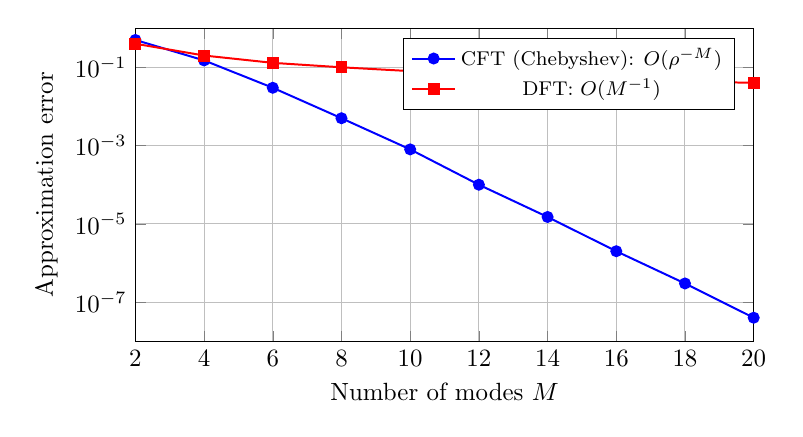
\begin{tikzpicture}[scale=0.9]
\begin{axis}[
    width=0.85\textwidth,
    height=6cm,
    xlabel={Number of modes $M$},
    ylabel={Approximation error},
    ymode=log,
    legend pos=north east,
    legend style={font=\footnotesize},
    grid=major,
    xmin=2, xmax=20,
    ymin=1e-8, ymax=1
]
\addplot[color=blue, mark=*, thick] coordinates {
    (2,0.5) (4,0.15) (6,0.03) (8,0.005) (10,0.0008) (12,0.0001) (14,1.5e-5) (16,2e-6) (18,3e-7) (20,4e-8)
};
\addlegendentry{CFT (Chebyshev): $O(\rho^{-M})$}

\addplot[color=red, mark=square*, thick] coordinates {
    (2,0.4) (4,0.2) (6,0.13) (8,0.1) (10,0.08) (12,0.067) (14,0.057) (16,0.05) (18,0.044) (20,0.04)
};
\addlegendentry{DFT: $O(M^{-1})$}
\end{axis}
\end{tikzpicture}
\caption{\textbf{Convergence rate comparison.} Approximation error versus number of modes $M$ for a function with jump discontinuities. CFT via Chebyshev expansion exhibits exponential convergence (blue), while standard DFT shows algebraic decay (red) due to Gibbs phenomenon. This exponential advantage enables CFT to capture high-frequency features that DFT misses even with many modes.}
\label{fig:convergence}
\end{figure}

\begin{figure}[p]
\centering
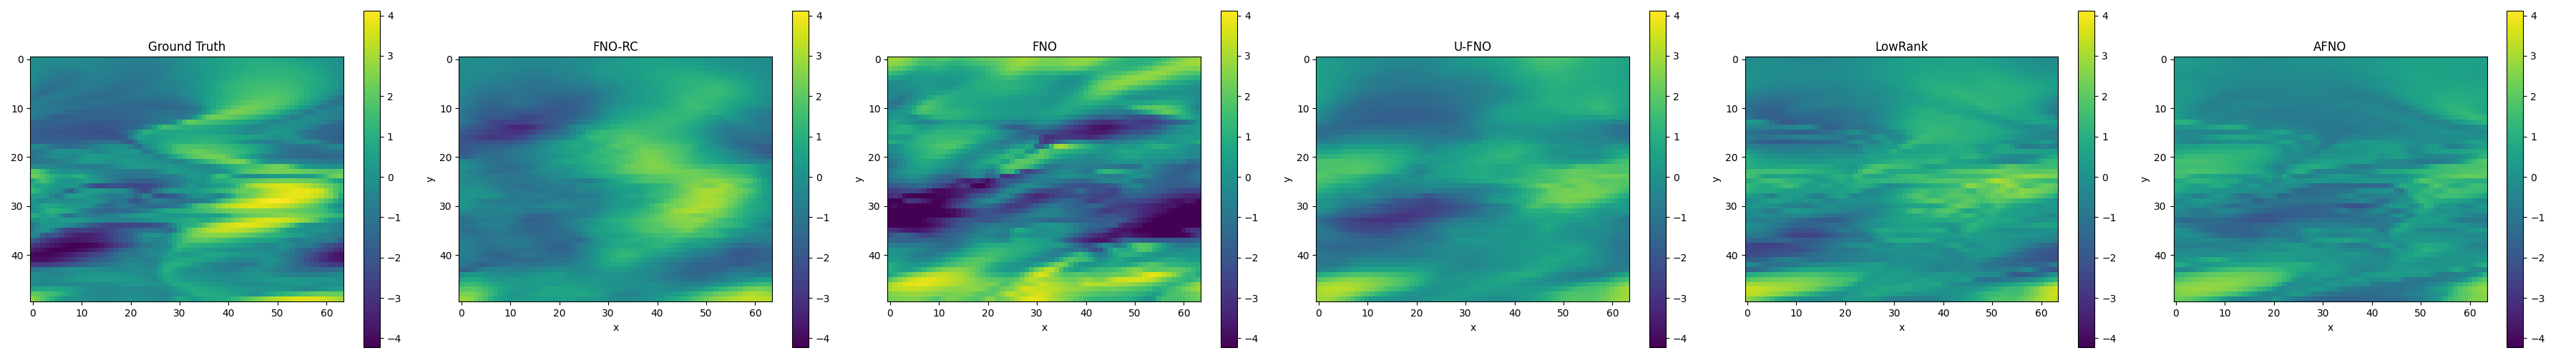
\includegraphics[width=0.9\textwidth]{../实验图/final_slice.png}
\caption{\textbf{Instantaneous flow field comparison at final time step.} Left to right: ground truth, FNO-RC prediction, standard FNO prediction. FNO-RC preserves fine-scale vortical structures and sharp velocity gradients; standard FNO shows excessive diffusion. Color scale denotes velocity magnitude.}
\label{fig:flow_instant}
\end{figure}

\begin{figure}[p]
\centering
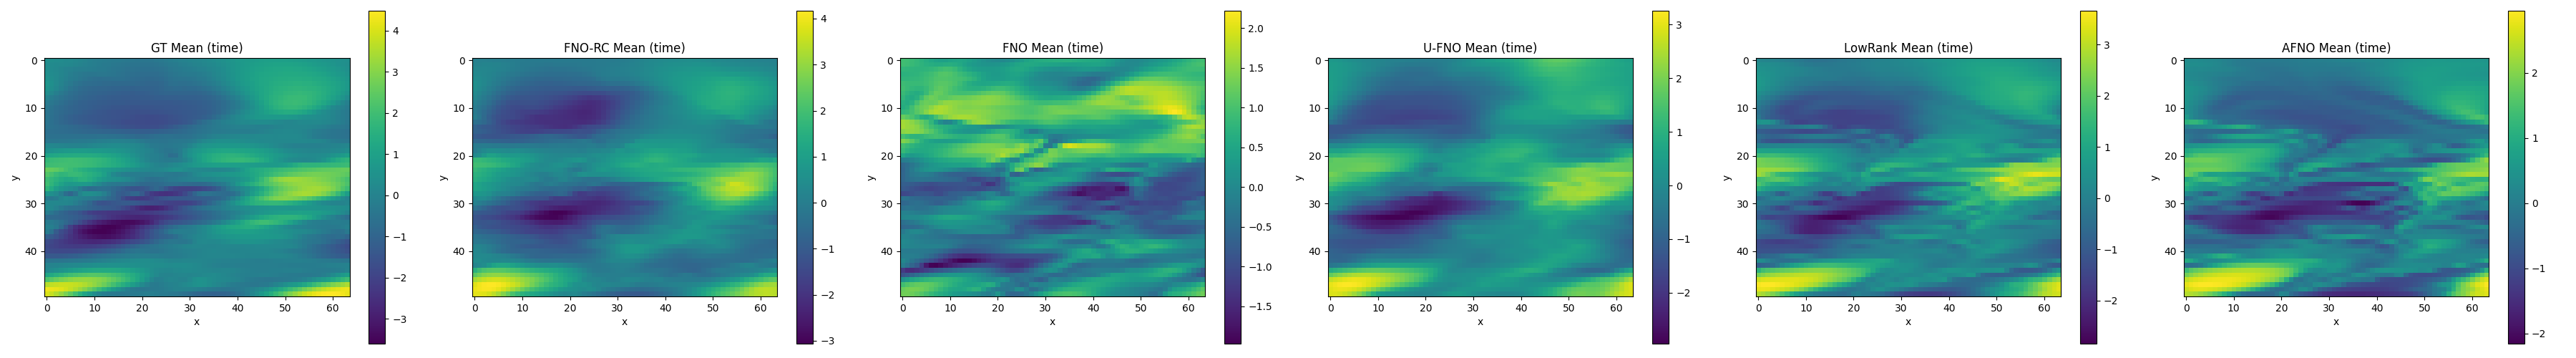
\includegraphics[width=0.9\textwidth]{../实验图/mean_time.png}
\caption{\textbf{Time-averaged velocity field comparison.} Left to right: ground truth, FNO-RC, standard FNO. FNO-RC maintains correct large-scale patterns with sharper statistics; standard FNO averages are overly diffused.}
\label{fig:flow_mean}
\end{figure}

\end{document}
